\documentclass[12pt,letterpaper]{exam}
\usepackage{amssymb,amsmath,amsfonts,amsthm,graphicx,ifthen,mathrsfs, wrapfig}
\usepackage{pgf,tikz}
\usetikzlibrary{arrows}

\oddsidemargin=0in
\evensidemargin=0in
\textwidth=6.5in
\topmargin=-1.0in
\textheight=9.0in
\parindent=0in


\newtheorem{problem}{Problem}
\newtheorem{claim}{Claim}
\newtheorem{theorem}{Theorem}
\newtheorem{definition}{Definition}

\begin{document}
\special{papersize=8.5in,11in}
\setlength{\pdfpageheight}{\paperheight}
\setlength{\pdfpagewidth}{\paperwidth}

\newcommand{\ud}{\,\mathrm{d}}
\pointsinmargin

Names: \underline{Chelsea Blake and Kelsey Mihachik}\\
Math 212 Fall 2015, Tennenhouse \\


\begin{center}
\textbf{HW 5, due 9/30/15}\\
\end{center}




[4, 5]
\begin{proof}$10n<n^2$ for $n\geq 11$ can be proven by induction.\\
Let's use the \textbf{base case} for $n=11$.
\begin{center}$10(11)<11^2$\\
$110<121$\end{center}
Under \textbf{inductive assumption}, let's say $n=k$ is true for all $k\geq 11$. So, $10(k)<k^2$.\\
For our \textbf{inductive step}, let's consider $n=k+1$ for all $k\geq 11$. Here we have:
\begin{center}$10(k+1)<(k+1)^2$\\
$10k + 10 < k^2+2k+1$\end{center}
If we know by assumption that $10(k)<k^2$, then the other terms in our inequality for $n=k+1$ will not make a difference. Suppose that they did. This would mean that the value '10' would have to make the left side greater than the right. However, we know this will not happen because the right side has an additional '2k' term, and we know that $k \geq 11$. Therefore, the left side will still be less than the right.
\end{proof}


[2]\\
The cube graph of of $Q_4$ will have 16 vertices: \\(0,0,0,0)(0,0,0,1)(0,0,1,0)(0,1,0,0)(1,0,0,0)\\ (0,0,1,1)(0,1,0,1)(0,1,1,0)(1,1,0,0)(1,0,0,1)(1,0,1,0)\\(1,1,1,0)(0,1,1,1)(1,0,1,1)(1,1,0,1)(1,1,1,1)\\
and edges where each of these differs in one spot exactly:\\
32 edges\\
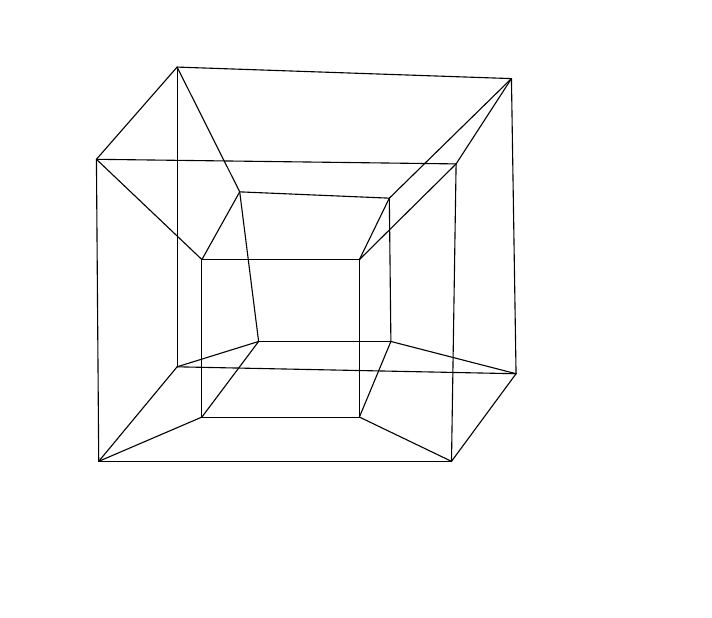
\begin{tikzpicture}[line cap=round,line join=round,>=triangle 45,x=1.0cm,y=1.0cm]
\clip(-2.212921999999994,-0.18889200000000628) rectangle (6.119138000000014,6.945268000000001);
\draw (0.,4.)-- (0.,2.);
\draw (0.,2.)-- (2.,2.);
\draw (2.,2.)-- (2.,4.);
\draw (2.,4.)-- (0.,4.);
\draw (2.,4.)-- (2.38,4.78);
\draw (0.,4.)-- (0.48,4.86);
\draw (0.48,4.86)-- (2.38,4.78);
\draw (2.38,4.78)-- (2.4,2.96);
\draw (2.,2.)-- (2.4,2.96);
\draw (0.,2.)-- (0.72,2.96);
\draw (0.72,2.96)-- (2.4,2.96);
\draw (0.72,2.96)-- (0.48,4.86);
\draw (-1.3397859999999977,5.273531999999999)-- (-1.3105039999999977,1.43759);
\draw (-1.3105039999999977,1.43759)-- (3.169642000000003,1.43759);
\draw (3.169642000000003,1.43759)-- (3.2282060000000032,5.214968);
\draw (3.2282060000000032,5.214968)-- (-1.3397859999999977,5.273531999999999);
\draw (-1.3397859999999977,5.273531999999999)-- (-0.31491599999999753,6.444812000000001);
\draw (3.2282060000000032,5.214968)-- (3.9309740000000035,6.298402000000001);
\draw (3.9309740000000035,6.298402000000001)-- (-0.31491599999999753,6.444812000000001);
\draw (3.9309740000000035,6.298402000000001)-- (3.989538000000003,2.550305999999997);
\draw (3.989538000000003,2.550305999999997)-- (3.169642000000003,1.43759);
\draw (-0.31491599999999753,6.444812000000001)-- (-0.31491599999999753,2.638151999999997);
\draw (-0.31491599999999753,2.638151999999997)-- (-1.3105039999999977,1.43759);
\draw (-0.31491599999999753,2.638151999999997)-- (3.989538000000003,2.550305999999997);
\draw (3.228206000000004,5.214968000000001)-- (2.,4.);
\draw (3.9309740000000026,6.298402000000002)-- (2.38,4.78);
\draw (3.169642000000003,1.43759)-- (2.,2.);
\draw (3.9895380000000036,2.5503059999999977)-- (2.4,2.96);
\draw (-1.3105039999999977,1.43759)-- (0.,2.);
\draw (-1.3397859999999981,5.273531999999999)-- (0.,4.);
\draw (-0.31491599999999587,6.444812)-- (0.48,4.86);
\draw (-0.3149159999999975,2.638151999999997)-- (0.72,2.96);
\end{tikzpicture}\\

\begin{proof}
For a graph $Q_n$, we can prove by induction that the number of vertices will be equal to $2^n$ and the edges will be equal to $2^{n-1}$ x $n$.\\
For our \textbf{base case}, let's use n = 2. A $Q_2$ graph would simply be a 2-dimensional square with 4 vertices and 4 edges.\\
\begin{center}Vertices = $2^2 = 4$\\Edges = $2^{2-1}$ x 2 = 4\\
\end{center}Our base case works.\\
Next for our \textbf{inductive assumption}, let's assume this is true for all $n=k$. So, vertices = $2^k$ and edges = $2^{k-1}$ x $k$.\\
Now for our \textbf{inductive step}, let's consider $n=k+1$. If the dimension of the graph raises by one, then the amount of vertices in the graph extends by twice the amount of vertices in the preceding dimension. If the preceding dimension was $k$ and it had $2^k$ vertices, then $Q_{k+1}$ will have twice that amount. Similarly, the number of edges increasing with each dimension would increase by a factor of k.\\
\begin{center} Vertices = 2 x $2^k$ = $2^1$ x $2^k$ = $2^{k+1}$\\
Edges = $2^{k}$ x $k+1=2^kk+2^k$
\end{center}
\end{proof}


[4,7]
\begin{proof}
$\sum_{i=0}^{n}3^i = \frac{3^{n+1}-1}{2}$ can be proven by induction.\\
For the \textbf{base case}, let's use $n=1$.
\begin{center}$\sum_{i=0}^{1}3^i = \frac{3^{1+1}-1}{2}$\\
$3^0 + 3^1 = \frac{3^2-1}{2}$\\
$1+3 = \frac{8}{2}$\\
$4=4$\\
\end{center}
Now by \textbf{inductive assumption}, let's assume true for $n=k$. So, we have $\sum_{i=0}^{k}3^i = \frac{3^{k+1}-1}{2}$.\\
With our \textbf{inductive step}, we can consider $n=k+1$, which would give us $\sum_{i=0}^{k+1}3^i$. Our proof will be complete if this is equal to $\frac{3^{k+1+1}-1}{2}$, or $\frac{3^{k+2}-1}{2}$.
\begin{center}
$\sum_{i=0}^{k+1}3^i$\\
=$\sum_{i=0}^{k}3^i$ + $3^{k+1}$\\
=$\frac{3^{k+1}-1}{2}$ + $3^{k+1}$\\
=$\frac{3^{k+1}-1+ 2(3^{k+1})}{2}$\\
=$\frac{3(3^{k+1})-1}{2}$\\
=$\frac{3^{k+1+1}-1}{2}$\\
=$\frac{3^{k+2}-1}{2}$
\\
\end{center}
\end{proof}




[4, 9]
\begin{proof}We can prove by induction that $K_n$ has $\frac{n(n-1)}{2}$ edges.\\
We will use $n=3$ as our \textbf{base case}. A $K_3$ graph will have three vertices, each connected to the other two vertices (essentially a triangle). Here, the number of edges is 3. If we plug in the number of vertices, 3, in for n, we get $\frac{3(3-1)}{2} = 3$. So our base case works.\\\\
For our \textbf{inductive assumption}, we can assume this is true for $n=k$, so the graph $K_k$ has $\frac{k(k-1)}{2}$ edges.\\\\
In our \textbf{inductive step}, let's consider $n=k+1$. If a vertex is added to the graph $K_k$, the number of vertices will be equal to $k+1$, and the number of edges will increase by $k$. The number of edges assumed for $K_k$ = $\frac{k(k-1)}{2}$, so the number of edges in the graph $K_{k+1}$ = $\frac{k(k-1)}{2} +k$. If our statement holds true, then this should be equal to $\frac{(k+1)k}{2}$.
\begin{center}
$\frac{k(k-1)}{2} +k$\\
$\frac{k(k-1)}{2} +\frac{2k}{2}$\\
$\frac{k^2-k+2k}{2}$\\
$\frac{k^2+k}{2}$\\
$\frac{(k+1)k}{2}$
\end{center}

\end{proof}




[4, 11]
\begin{proof}
We can use induction to prove that $((n+1)!)^n \leq 2!4! \ldots (2n)!$.\\
Let's use $n=1$ as our \textbf{base case}. $((1+1)!)^1 \leq (2(1))!$. $2 = 2$, so our base case works.\\\\
Now by \textbf{inductive assumption}, let's assume this is true for $n=k$, so that $((k+1)!)^k \leq 2!4! \ldots (2k)!$.\\\\
With our \textbf{inductive step}, let's consider $n=k+1$. The left side of the inequality would then be $((k+2)!)^{k+1}$, while the right side would be the same thing as saying $((k+1)!)^k$ x $[2(k+1)]$.
\begin{center} $((k+2)!)^{k+1}$  $\leq$  $((k+1)!)^k$ x $[2(k+1)]!$\\
$((k+2)!)^{k}$ x $((k+2)!)^1$  $\leq$  $((k+1)!)^k$ x $(2k+2)!$\\
divide both sides by $(k+1)!^k$\\
$1!^k$ x $(k+2)!$  \leq  $(2k+2)!$\\
$(k+2)!$  \leq  $(2k+2)!$\\
$k+2$  \leq  $2k+2$\\
$k$  \leq  $2k$\\
$1$  \leq  $2$\\
\end{center}

Since the inequality at the end is a true statement, our proof is complete.

\end{proof}\\



[4, 13]
We can prove $n!<n^n$ as long as $n\geq 2$ by induction.\\
For our \textbf{base case}, let's test $n=2$.
\begin{center}$2! < 2^2$\\
$2! < 4$
\end{center}Here, we see the base case works. Now for our \textbf{inductive assumption}, let's assume this is true for all $n=k$. So, $k!<k^k$ as long as $k\geq 2$.\\
In our \textbf{inductive step}, let's consider $n=k+1$. The inequality would then become:
\begin{center}$(k+1)!<(k+1)^{k+1}$ as long as k+1 $ \geq 2$, or k $\geq 3$\\
\end{center}
We can break down this inequality by noticing that (k+1)! is equal to the quantity k! times (k+1).
\begin{center}$k!(k+1)<(k+1)^{k+1}$\\
$k!(k+1)<(k+1)^{k}(k+1)^1$\\
divide both sides by (k+1)\\
$k!<(k+1)^k$
\end{center}
We know this inequality is true, due to our inductive assumption. In our assumption, we said $k!<k^k$ as long as $k\geq 2$. Well, the only way this equality differs from our assumption is that it is now $(k+1)^k$. If we know the value of k has to be at least 2, then we know there is no value of k that exists which would make k+1 less than k. That being said, the right side of the inequality is still greater than the left, and our statement is proven.\\\\





\question[4, 17]
\emph{Show that every tree (a connected graph with no cycles) is bipartite using induction.}
\begin{proof}
\\
A tree is a graph in which any two vertices are connected by only one edge. For the \textbf{base case} we will use a tree with two vertices, this tree only has one edge and therefore can be seperated into two subgroups connected by an edge. This graph is bipartite.
\\
The \textbf{inductive assumption } states that there exists a tree with $k$ vertices that is bipartite.
\\
The then must show in the \textbf{inductive step} that there exists a tree with $k+1$ vertices that is bipartite. We know that a tree with $k$ graphs can be split into two subsections by the inductive assumption. 

\end{proof}

[4, 20]
\begin {proof}
The sum of the interior angles of any $n$-gon (a polygon with $n$ sides) is $\pi (n-2)$ can be shown using the induction proof. The \textbf{base case} for this problem will be where $n=3$ because $3$ is the smallest number of sides a $n$-gon can have. the sum of the interior angles of a 3-sided polygon is $180^o$ or $\pi$ radians (this problem will be worked through in radians). we then see that $\pi=\pi(3-2)$ or $\pi=\pi$ and our base case works. 
\\
Next, for the \textbf{inductive assumption} we assume that the sum of interior angles of a  $k$-gon is $\pi (k-2)$ for any $k \ge 3$. 
\\
Finally, for our \textbf{inductive step} we show that this is true for $k+1$. Lets say we have a $k+1 k$-gon and we draw a line segment connecting two edges  that are sepzrated by one edge making a $k$-gon and a triangle (see figure below). We can then say that the sum of interior angles of the $k+1$-gon is simply the sum of the interior angles of the $k$-gon plus a triangle. From the base case we know that a triangle (or 3-sided polygon) has a sum of $\pi$ and that $\pi=\pi(3-2)$. We also know from the inductive assumption that the sum of a $k$-gon is $\pi (k-2)$. We can then conclude that a $k+1$-gon has a sum of interior angles of $\pi (k-2) + \pi=\pi((k+1)-2)$. So a $k+1$-gon has a sum of interior angles of $\pi((k+1)-2)$ which is exactly what we wanted to show.
\\
\definecolor{qqqqff}{rgb}{0.,0.,1.}
\begin{tikzpicture}[line cap=round,line join=round,>=triangle 45,x=1.0cm,y=1.0cm]
\clip(2.92,5.2) rectangle (11.86,11.08);
\draw (5.84,8.3)-- (5.5,7.84);
\draw (5.5,7.84)-- (5.48,7.14);
\draw (5.48,7.14)-- (5.5,7.16);
\draw (5.5,7.16)-- (5.86,6.6);
\draw (5.86,6.6)-- (6.3,6.56);
\draw (6.3,6.56)-- (6.72,6.6);
\draw (6.72,6.6)-- (7.,7.);
\draw (7.,7.)-- (7.02,7.42);
\draw (7.02,7.42)-- (6.82,7.94);
\draw (6.82,7.94)-- (6.48,8.38);
\draw (6.48,8.38)-- (5.84,8.3);
\draw (9.26,8.44)-- (8.92,7.98);
\draw (8.92,7.98)-- (8.9,7.28);
\draw (8.9,7.28)-- (8.92,7.3);
\draw (8.92,7.3)-- (9.28,6.74);
\draw (9.28,6.74)-- (9.72,6.7);
\draw (9.72,6.7)-- (10.14,6.74);
\draw (10.14,6.74)-- (10.42,7.14);
\draw (10.42,7.14)-- (10.44,7.56);
\draw (10.44,7.56)-- (10.24,8.08);
\draw (10.24,8.08)-- (9.9,8.52);
\draw (9.9,8.52)-- (9.26,8.44);
\draw (9.26,8.44)-- (10.24,8.08);
\begin{scriptsize}
\draw [fill=qqqqff] (5.84,8.3) circle (1.5pt);
\draw [fill=qqqqff] (5.5,7.84) circle (1.5pt);
\draw [fill=qqqqff] (5.48,7.14) circle (1.5pt);
\draw [fill=qqqqff] (5.5,7.16) circle (1.5pt);
\draw [fill=qqqqff] (5.86,6.6) circle (1.5pt);
\draw [fill=qqqqff] (6.3,6.56) circle (1.5pt);
\draw [fill=qqqqff] (6.72,6.6) circle (1.5pt);
\draw [fill=qqqqff] (7.,7.) circle (1.5pt);
\draw [fill=qqqqff] (7.02,7.42) circle (1.5pt);
\draw [fill=qqqqff] (6.82,7.94) circle (1.5pt);
\draw [fill=qqqqff] (6.48,8.38) circle (1.5pt);
\draw [fill=qqqqff] (9.26,8.44) circle (1.5pt);
\draw [fill=qqqqff] (8.92,7.98) circle (1.5pt);
\draw [fill=qqqqff] (8.9,7.28) circle (1.5pt);
\draw [fill=qqqqff] (8.92,7.3) circle (1.5pt);
\draw [fill=qqqqff] (9.28,6.74) circle (1.5pt);
\draw [fill=qqqqff] (9.72,6.7) circle (1.5pt);
\draw [fill=qqqqff] (10.14,6.74) circle (1.5pt);
\draw [fill=qqqqff] (10.42,7.14) circle (1.5pt);
\draw [fill=qqqqff] (10.44,7.56) circle (1.5pt);
\draw [fill=qqqqff] (10.24,8.08) circle (1.5pt);
\draw [fill=qqqqff] (9.9,8.52) circle (1.5pt);
\end{scriptsize}
\end{tikzpicture}
\end{proof}


[4, 21]
The equation $$1+3+6+10+ \cdots +\frac{n(n+1)}{2}=\frac{n(n+1)(n+2)}{6}$$ can be rewritten as $\sum^{n}_{i=1}\frac{i(i+1)}{2}$ = $\frac{n(n+1)(n+2)}{6}$\\\\

\begin{proof}
This can be proven for all positive integers using induction. For our base case, let's try $n=1$.\\
\begin{center}Left side is: $\sum^{n}_{i=1}\frac{1(1+1)}{2} = \sum^{n}_{i=1}1 = 1$\\
Right side is: $\frac{1(1+1)(1+2)}{6} = \frac{(2)(3)}{6} = 1 $
\end{center}Our base case works. Now for our \textbf{inductive assumption}, let's assume this is true for all $n=k$. So, $\sum^{k}_{i=1}\frac{i(i+1)}{2}$ = $\frac{k(k+1)(k+2)}{6}$.\\
In our \textbf{inductive step}, let's consider $n=k+1$. The sum $\sum^{k+1}_{i=1}\frac{i(i+1)}{2}$ would be equal to $\sum^{k}_{i=1}\frac{i(i+1)}{2}$ plus the component $\frac{(k+1)(k+2)}{2}$ Let's plug in our value from our assumption for $\sum^{k}_{i=1}$:\\
\begin{center}
$\sum^{k+1}_{i=1}$= $\frac{k(k+1)(k+2)}{6}$ + $\frac{(k+1)(k+2)}{2}$\\
= $\frac{k(k+1)(k+2)}{6}$ + $\frac{3(k+1)(k+2)}{6}$\\
= $\frac{(k+3)(k+1)(k+2)}{6}$\\
\end{center}Since we received the value we were looking for, the statement is proven.
\end{proof}\\\\\\

[4,23]
\begin{proof}
\\
In this proof we must show that any  $2^n \times 2^n$ grid missing \emph{any} square will come out to a number divisible by 3. We know that  $2^n \times 2^n=2^{2n}$ and our equation $2^{2n}-1$ must be divisible by 3.For the \textbf{base case} we use 1 and get $2^{2}-1=4-1=3$ 3 is divisible by 3 so our base case works.
\\
We then look at \textbf{inductive assumption} that states that there exists some $k$ such that any $2^k \times 2^k$ grid missing any square can be tiled with L-shaped tiles. in other words $2^{2k}-1=$ a number divisible by 3.
\\
For our \textbf{inductive step} we must find that $2^{2k+2}-1$ is also equal to a number divisible by 3. 
\\
$2^{2k+2}-1= ((2^{2k} \times 2^2) -1 = (2^{2k} \times 4) -1 $\\
=$2^{2k}+2^{2k}+2^{2k}+2^{2k} -1$\\
We know that $(2^{2k}-1)$ is divisible by 3 by the inductive assumption. We are then left with $3(2^{2k})$ and anything multiplied by 3 can then be divided by 3, therefore we proved that $2^{2k+1}-1$ is also equal to a number divisible by 3. 
\end{proof}


\end{document}
